\section[Elektronová mikrosonda]{Elektronová mikrosonda}

= Elektronový mikroskop

\subsection{Princip}

Jedná se v zásadě o elektronový mikroskop s kombinací RTG analýzy (obsahuje modul pro detekci a analyzování RTG).

Elektronová mikroskopie, neboli SEM (Scanning Electron Microscopy = skenovací/rastrovací elektronová mikroskopie) obsahuje soubor metod/možností, co lze v materiálu zkoumat, a to na základě detekce různých signálů. Urychlené elektrony bombardují povrch vzorku a elektronový paprsek z elektronového mikroskopu je fokusován na velmi malou plochu.

Základní komponenty elektronového mikroskopu jsou: \begin{itemize}
    \item Elektronové dělo 
    \item[-] TEG (Thermionic Emission Gun, W, LaB$_6$) -- katoda je zahřáta na několik tisíc stupňů K, emituje termoelektrony. Menší rozlišení kvůli velikosti emitoru, ale je levnější.
    \item[-] FEG (Field Emission Gun, velmi tenký krystal W) -- využívá se elektronového tunelování k emsisi elektronů o velmi dobré koherentnosti, tedy mám velmi dobré rozlišení, stačí pokojová teplota. Problém je, že je drahá a krystal kontaminují plyny vzniklé ionizací elektrony.
    \item[-] SEG (Schottky Emission Gun, W + ZrO potah) -- podobný princip jako FEG, ale nemá takovou adsorpci plynů a má velmi silný proud. Rozlišení skoro tak dobré jako FEG, je to vlastně FEG za vysokých teplot.
    \item Série elektromagnetických čoček -- usměrňuji svazek elektronů a to jak ve smyslu urychlení, tak i co se týče jeho průměru. Také ho navádí, resp. umožňuje skenování povrchu vzorku.
    \item Systém vakua
    \item Detektory pro záznam příslušného signálu
    \item Systém pro zpracování signálu a jeho vykreslení včetně PC
\end{itemize} 


\begin{figure}[H]
    \centering
    \includegraphics[width=0.7\linewidth]{img/elektronová mikrosonda.png}
    \caption{Elektronová mikrosonda}
\end{figure}

Rozlišení a rozlišovací schopnost, stejně jako přiblížení, jsou značně lepší (cca 1000x) a větší než v případě LOM, což je dáno právě použitými elektrony. Rozlišovací schopnost je dána vlnovou délkou elektronů, která je značně kratší (de Broglie ~ 0,01 nm). 

Vlnová délka závisí urychlovacím napětí.

\textbf{Co vzniká při dopadu elekttonů na povrch zkoumaného vzorku:}

\begin{itemize}
    \item BSE -- jedná se o elektrony, jež dopadají a odráží se od povrchu vzorku, nebo prochází do materiálu do určité hloubky. Zde se srážkami odráží, tvoří SE a pak se v materiálu odraží a letí zpět, čímž se dostanou zpátky do sondy.
    \item[-] Slouží například pro fázovou analýzu.
    \item[-] Lehké atomy méně odráží elektrony, což se projeví tmavým obrazem. Naopak těžší atomy lépe odráží a obraz je pak světlejší.
    \item  SE -- jedná se o sekundární elektrony, neboli elektrony, které vznikají v důsledku BSE, které je vyráží z atomů v materiálu.
    \item[-] Zobrazení povrchu vzorku, často jsou detekovány scintilačním detektorem. Podávají informaci o rovnosti materiálu. Pokud je materiál vlnity a hrubý, tak absorbuje více elektronů a proto je obraz tmavý. Pokud je hladký a rovný, tak se více elektronů odráží a proto je povrch světlý a lesklý.
    \item Charakteristické RTG záření -- při vyražení elektronu ze slupky K nebo L dochází k zaplnění díry z vyšší slupky. Rozdíl energií je vyzářen v podobě charakteristického RTG záření, jež následně detekujeme. Tím máme možnost dělat analýzu chemického složení zkoumaného materiálu.
    \item[-] Podává info o povrchové koncentraci prvku. Mohu si například zvolit v jakém směru chci měřit, což je užitečné, pokud mám materiál z více vrstev (např. pokrytí paliva). V druhém případě si mohu dělat i celé mapy daného povrchu s koncentrací jednotlivých prvků.
    \item Katodoluminiscence (vznik viditelného záření)
    \item AE -- Augerovy Elektrony
\end{itemize}

\subsection{Typy elektronového mikroskopu:}

\begin{itemize}
    \item \textbf{SEM} (Scaning Electron Microscopy):
    \item[-] Urychlené a usměrňované elektrony skenují povrch zkoumaného vzorku a způsobují tvorbu SE, BSE, RTG, Katodoluminscence a AE. Signály jsou poté zaznamenány příslušným detektorem a analyzovány.
    \item[-] SEM poskytuje trojrozměrné obrazy povrchu a je užitečný při studiu morfologie vzorků.
    \item[-] Zobrazení povrchu pomocí sekundárních elektronů nebo zpětně odražených elektronů.
    \item[-] Urychlovací napětí: 0,1-30 keV
    \item \textbf{TEM} (Transmission Electron Microscopy):
    \item[-] Zobrazení pomocí prošlých elektronů.
	\item[-] Urychlovací napětí (100-400 keV) musí být dostatečně velké, aby elektrony měly dostatečnou energii a prošly skrz.
    \item[-] Tenké vzorky, do kterých se pak dělá malinká dírka skrz kterou projdou elektrony (s tou dírkou si nejsem jistý). 
\end{itemize}

\underline{Pozn.1:} Abych mohl dělat elektronovou mikroskopii, tak je potřeba, aby zkoumaný materiál byl vodivý, resp. alespoň povrch, jelikož penetrace a vznik všech těch věcí je řádově jednotky, max. 10-15 mikronů. Nevodivé vzorky se tak buď oblepují ze stran vodivou páskou, a nebo se pokrývají tenkou vrstvou Al, či Au.

\underline{Pozn.2:} Kromě klasické elektronové mikroskopie SEM, tak je ještě EBSD -- Electron Backscatter Difraction, který nám dává mapy s natočením jednotlivých zrn ve struktuře. EDS a WDS jsou energiově a vlnově disperzní spektrometrie a TEM je transmisivní elektronová mikroskopie, kdy elektrony prochází skrze velmi tenký vzorek (elektrony jsou hodně urychleny -- 60 keV $\rightarrow$ u SEM je to okolo 15-30 keV). TEM má lepší rozlišení a to až na úrovni jednotlivých atomů.

\subsection{Využití}

\begin{itemize}
    \item Kvantitativní analýza prvkového složení u zkoumaného materiálu na mikro měřítku.
    \item Umožňuje měřit prvky těžší než Li (i stopová množství, min. 100 ppm) s přesností okolo 1-2 \%.
    \item Společně s elektronovým mikroskopem jde o nástroj pro zkoumání nejen prvkového složení a jejich koncentrace, ale také topografie materiálu, natočení zrn, fázové složení apod.
\end{itemize}

\begin{figure}[H]
    \centering
    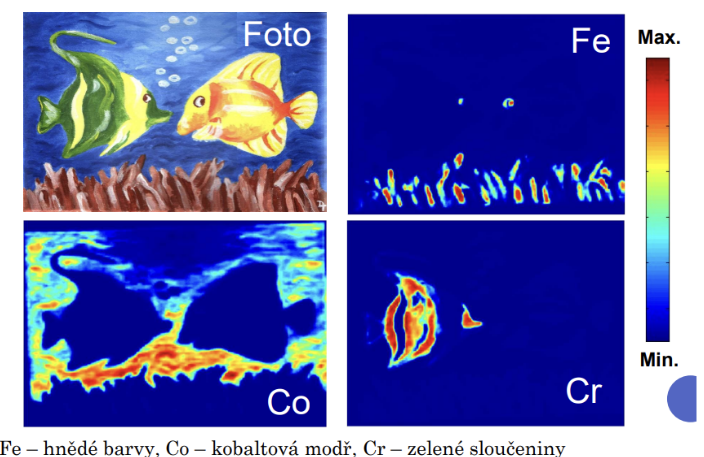
\includegraphics[width=0.6\linewidth]{img/využití elektronové mikrosondy v praxi.png}
    \caption{Využití elektronové mikrosondy v praxi}
\end{figure}

\subsection{Výhody a nevýhody elektronového mikroskopu}

\textbf{Výhody:}
\begin{itemize}
    \item Vysoké rozlišení -- pracují s elektromagnetickými čočkami namísto optickými, což umožňuje dosahovat mnohem vyššího rozlišení než světelné mikroskopy. To je zvláště užitečné při studiu malých struktur na mikro a nano úrovni.
    \item Velké zvětšení -- díky schopnosti pracovat s krátkou vlnovou délkou elektronů mohou elektronové mikroskopy dosáhnout velkých zvětšení.
    \item Podrobný pohled na vnitřní struktury -- TEM umožňuje podrobný pohled na vnitřní struktury vzorků, což je užitečné pro studium buněčné a materiálové biologie.
    \item Trojrozměrný obraz: SEM poskytuje trojrozměrný obraz povrchu vzorku, což je užitečné pro studium morfologie.
    \item Široká škála aplikací - materiálový výzkum, umění, archeologie, částečně i geologie a biologické předměty.
\end{itemize}

\textbf{Nevýhody:}
\begin{itemize}
    \item Vysoké náklady -- elektronové mikroskopy jsou nákladné na pořízení, údržbu a provoz.
    \item Složitá obsluha -- obsluha elektronových mikroskopů vyžaduje odborné znalosti a dovednosti a proto vyžaduje školený personál.
    \item Vakuové prostředí -- pro správnou funkci je nutné pracovat ve vakuovém prostředí, což může omezit studium některých živých vzorků.
    \item Příprava vzorků -- příprava vzorků může být složitá a vyžaduje speciální postupy, jako je například nástřik tenké vrstvy kovu pro TEM.
    \item Rozměry a hmotnost -- elektronové mikroskopy jsou obvykle velké a těžké zařízení, což omezuje jejich přenosnost a umístění do menších laboratoří.
\end{itemize}